\chapter{Related Work}

\epigraph{\textit{If I have seen further, it is by standing on the shoulders of Giants.}} {Issac Newton}

\newpage
\section{Introduction}
\section{Theoretical concepts}\label{Theoretical}

\subsection{Bulk Synchronous Parallel Paradigm}\label{BSP}
In \cite{valiant1990bsp}, \textit{Leslie G. Valiant} introduced the bulk-synchronous parallel paradigm as a bridging model between software and hardware for parallel computing. He argued that such a model is analogous to the \textit{Von Neumann} model and would get the same success as this last.
A Bulk-Synchronous Parallel computer combines three attributes : 
\begin{itemize}
    \item a number of \textbf{components}, each performing processing and/or memory functions,
    \item a \textbf{router} that delivers messages point to point between pairs of components,
    \item facilities for \textbf{synchronizing} all or a subset of the components at regular intervals of $L$ time units where $L$ is the Periodicity parameter.
\end{itemize}

A BSP machine can be implemented using the well-known communication interface: Massage Passing Interface (MPI), where the components are defined as a set of $P$ processes that share a common communicator. Each process has its separate local memory, performs a set of computations on its local data, and then exchanges some results with other processes. A local/global synchronization is performed periodically. Such a paradigm suits very well the scientific applications where models are regular. The global domain is decomposed statically and explicitly within the processes. Each process has its local buffers updated as the simulation progresses, and parts of those buffers are exchanged with a subset of processes when needed. In this work, we will focus on the MPI implementation of the BSP paradigm.

%Not only does the paradigm seem natural to design regular applications (which is the case for high-performance simulations), but its implementations (specifically using MPI) respond to a critical requirement of HPC applications, which is the high performance itself.

%MPI is already a very known programming model. We will not detail it here. However, we will summarize the most important characteristics that have made it extremely successful since its appearance.

Unlike several programming models that introduce new complex concepts, MPI was built in relatively small, well-defined, and forward-looking concepts\cite{traff_recent_2012}. In the MPI-1 standard, an MPI process runs a program in his private address space and can communicate either through point-to-point message passing with another process or through collectives. The standard has been then extended in several ways however, using MPI may only require knowing a few concepts. In addition to the strong base of MPI, it was designed to work with other tools. This characteristic is vital because the complexity of software and hardware keeps increasing. It also supports component-oriented software, thanks to communicators and groups, which is very important in designing modular or hierarchical code. Moreover, MPI is a complete model that can be used to write any parallel algorithm and is portable and can be used on platforms ranging from a laptop to a supercomputer\cite{goos_learning_2001}. All those characteristics make MPI perfectly fit high-performance applications and be the most used model in HPC.

Note that in MPI, the resource allocation and scheduling are managed explicitly; while this is not a big issue for regular algorithms, it can quickly become complicated to manage for irregular ones.

\subsection{Distributed Task-based Programming}

Despite MPI's success, it may not be the most suited model to parallelize irregular algorithms. This category of problems is characterized by irregular data structure and control patterns, and using static decomposition to parallelize them is not trivial. Higher-level programming models such as task-programming reduce this complexity by cutting the computation into a set of tasks then dynamically scheduling them. In this work, we will focus in distributed task-based programming. 

%\cite{kooburat_extending_nodate} extend shared memory to distributed 


In the task-based paradigm, we define three main attributes as well :
\begin{itemize}
    \item a number of \textbf{stateless tasks}, each task performs a given job. It is defined as a sequence of instructions. A task can be either fine-grained or of a coarser granularity, it may have one or more inputs and outputs,
    \item \textbf{dependencies} between tasks. A task can only be executed when all its dependencies are resolved,
    \item an \textbf{engine} that manages and \textbf{schedules} the execution of those tasks on a set of physical processes.
\end{itemize}

\textbf{Actor} is another concept that has emerged in several task-based systems. It is a stateful entity, it has internal attributes 
that may be immutable, when receiving messages from the environment it may react by changing its internal state or/and send responses. 

One of the main motivations for introducing such a model is to create higher-level abstractions that make the design and implementation of parallel algorithms easier. The resource and the task scheduling are managed by a runtime, implicitly from the user's point of view. The task-based models can be less efficient in terms of performance compared to BSP-based models due to the overheads that may be introduced during runtime. However, they widely increase productivity with the simplicity they introduce in designing and maintaining non-trivial applications.   

In this work, we have chosen the \dask distributed framework, and we will present in detail its architecture, task and data management and internal scheduling in section~\ref{sec:dask.distributed} 

\section{In Situ Paradigm}\label{sec:insitu}

The in situ paradigm stands for processing the data generated by a simulation code as close as possible to when and where they are generated. The paradigm has been used first for visualization\cite{InSituLiuMa:2007} and then extended for general-purpose processing. There are several ways to perform in situ analysis, either by time or space sharing with the simulation processes. They can share the same thread, the same process, or just the same node; the processing in those cases is called In situ. If they only share the same platform, and the data is sent to staging nodes, then we say in-transit processing.

In traditional data processing workflows, the data is first written to disk and then read back for post-processing in separate workstations. With the widening gap between CPU performance and IO bandwidth, such a workflow is not possible anymore in some fields. The in situ paradigm is a good alternative as it allows bypassing disk access, thus avoiding the IO bottleneck.  

[limitations] on garde pas tous et on ne sait pas forcement ce qu on veut faire 


\subsection{In Situ Frameworks}

%ADIOS I, II, Damaris, FlowVR, decaf, bredala, filtring, smartsim, 

The in situ paradigm has been applied first to scientific visualisation\cite{InSituLiuMa:2007}. Thus, most scientific visualization frameworks that are meant for high-performance computing support in situ visualization. Paraview~\cite{ahrens_paraview_2005} and Visit~\cite{childs_visit_nodate} both support in situ visualization thanks to the Catalyst~\cite{catalyst11} and Libsim~\cite{libsim11} extensions, respectively.

Due to the efficiency of the in situ, it emerged quickly to general-purpose usage with a set of infrastructures and frameworks. Sensei~\cite{ayachit_sensei_2016}, a generic in situ interface that focuses on having a unified API to instrument the simulation codes and making use of external tools to handle data. Its architecture is built on three main components, a \textbf{data adaptor} from the simulation side, an \textbf{analysis adaptor} from the analytics side and a bridge between the two that can be, for instance, the vtk data model. Sensei already supports several backends, such as Alpine/Ascent/vtkm\cite{Larsen-alpine-isav17,moreland_vtk-m_2016}, ADIOS\cite{lofstead_insights_2013_adios,boyuka_transparent_2014_adios} as well as for Paraview/Catalyst and Visit/libsim. The previously mentioned, Ascent\cite{Larsen-alpine-isav17} uses conduit\cite{larsen_strawman_2015} as a bridge data model between a data producer and consumer. 

Decaf\cite{dreher_decaf_2017}, a dataflow middleware for in situ workflows, proposes the concept of a \textit{link} to couple a producer and a consumer of data. The \textit{link} is deployed in a set of separate resources where operation on the data structure can be performed. Bredala\cite{dreher_bredala_2016} is built on Decaf; it provides an API to construct a data model with enough information to keep its semantics while splitting and merging. The work on decaf and Bredala was a strong base to propose a new concept to extract needed data for analytics automatically at the producer, called contracts\cite{mommessin_automatic_2017}.

SmartSim\cite{smartsim_2022, site_introduction_smartsim} provides a different way to couple running simulations with analytics, mainly IA models, at runtime; It uses the Redis\cite{redis} im-memory key-value data store. The Smartsim architecture is built on two main components: the SmartSim Infrastructure Library and SmartRedis. The first is a python-based workflow library that facilitates the dynamic execution of HPC simulations and ML infrastructure, and the second consists of a lightweight client library used in applications to communicate with infrastructure started by SmartSim\cite{smartsim_2022}. 

We also find several tools that were meant for IO management and then adapted for in situ analytics. ADIOS1\cite{lofstead_insights_2013_adios,boyuka_transparent_2014_adios} and ADIOS2\cite{godoy_adios2_2020}, Damaris\cite{dorier_damaris_2012} or 
Dataspaces\cite{docan_dataspaces_2012} are examples of frameworks in that category. FlowVR\cite{dreher_flexible_2014} on its side was developed for virtual reality and has been adapted to support both in situ and in transit analytics.
 
All of these tools rely on static parallelization. The tasks of the analysis workflow are mapped to compute resources statically.
This often leads to high performance but requires the user to control this mapping explicitly. The underlying transport layer is often based on MPI(except for SmartSim based on tcp\cite{site_introduction_smartsim}), simplifying the coupling with the simulation code also based on MPI, or the introduction of an analysis algorithm parallelized with MPI in the workflow. 



\subsection{Task-based Programming in In Situ Workflows}

Task-based programming in shared memory is commonly used today in scientific applications to efficiently leverage nodes architecture, using OpenMP\cite{openMP} or Intel TBB\cite{Robison2011tbb}. Both have been used in the context of in situ processing. TBB has been used in TINS\cite{yokota_tins_2018} to dynamically distribute the simulation and the analytics tasks to the available cores. The dynamic and work-stealing scheduler of TBB improves performance as cores are not assigned exclusively to analysis or simulation workload. OpenMP is similarly used in Goldrush\cite{zheng2013goldrush}, where idle cores unused by the running simulations, can be used to run in situ analytics.   
Sun et, al.~\cite{staging_2016_manish} propose an asynchronous coupling of task-based scientific workflows by relying on  dataspaces\cite{docan_dataspaces_2012} as a staging area. Both simulation and in situ analytics are parallelized in tasks. 


\subsection{Big Data Frameworks in In Situ Workflows}

In addition to BSP, Big Data models are built on several other programming models such as functional, SQL-based, Actor model and the current defacto framework/model for writing data-centric applications is Map-reduce\cite{Wu2017}. A few attempts to use this last alongside the in situ paradigm, for instance, SMART\cite{wang_smart_2015} proposes a map/reduce interface for programming in situ analysis on top of MPI/OpenMP. And \cite{zanuz_-transit_2018_flink} takes benefit of Flink stream processing support for enabling in transit analysis.
But the model provides a loose control on data partitioning that is not well adapted to support efficient parallelization of patterns such as stencil computations\cite{arrayUDF-SC2018} or large-scale linear algebra.


\section{Distributed Task-based Frameworks}

The task-based programming paradigm 

%Dask Parsl Ray pycompss starpu parsec Legion/pygion



\section{Used Tools}




\subsection{\dask Distributed}\label{sec:dask.distributed}
\subsubsection{Overview}
\dask distributed has been chosen to be used as a task-based framework in this work.  
It has three main components: one or more clients, a scheduler, and one or more workers. The client is the entry point to the \dask cluster; it represents an interface between the end-user and \dask. 
The user writes an almost sequential code using the available APIs in \dask. A task graph can be constructed using written functions based on low-level \texttt{Delayed} and \texttt{Future} APIs, or it can be generated automatically by using the available high-level APIs such as \texttt{dask.array} (see listing~\ref{listnumpy} and listing~\ref{listdask}). The task graph is then submitted to the scheduler by calling specific functions such as \texttt{compute} and \texttt{persist}.    

The scheduler analyses the task graph and checks any connected workers; if so, it sends the ready tasks to the idle workers. The workers are multi-threaded processes that perform the computations, store and share the data. 

The source of the data in \dask is usually a storage system. A classical post hoc workflow can be illustrated in figure~\ref{figdaskarchi}. The code in listing~\ref{listdask} will be run following these steps. The client connects first to the scheduler. It reads the metadata from the parallel file system regarding the HDF5 file \texttt{"data.hdf5"} and the dataset \texttt{"dataset1"}. A \texttt{dask.array} object is created using the descriptor. By calling \texttt{mean} method, the task graph is created. Concretely, the \texttt{numpy.mean} function is called on each chunk, and an aggregation tree is created to compute the mean of the whole array. The task graph is submitted to the scheduler, which sends the tasks without any dependencies to the workers first. In this case, those tasks are \texttt{getitem} tasks that read data from the file. 

Note that in \dask, it's only at this stage that the concrete dataset is read, which makes it possible to process data larger than one node's memory in parallel.

Once all the tasks are computed, the result is returned to the client.

\begin{lstlisting}[float, label=listnumpy, language=python, caption=Sequential post hoc mean using numpy]
import numpy as np
import h5py
# Load data from HDF5
dataset1 = h5py.File('data.hdf5',mode='r')['dataset1']
# Compute the mean of the array
computed_mean = np.array(dataset1).mean()
print("Computed mean : ", computed_mean)
\end{lstlisting}

\begin{lstlisting}[float, label=listdask, language=python, caption=Parallel post hoc mean with \dask. Lines differing from the analysis of Listing~\ref{listnumpy} are highlighted]
|\hlline|import dask.array as da
import h5py
|\hlline|# Connect to Dask
|\hlline|client = dask.distributed.Client(address)
# Build a lazy array descriptor from HDF5
dataset1 = h5py.File('data.hdf5',mode='r')['dataset1']|\label{post:hdf5}|
|\hlline|dataset1 = da.from_array(dataset1, chunks=(1,4096,4096))|\label{post:chunk}|
computed_mean = dataset1.mean.compute()
print("Computed mean : ", computed_mean)
\end{lstlisting}

\begin{figure}[tb]\centering
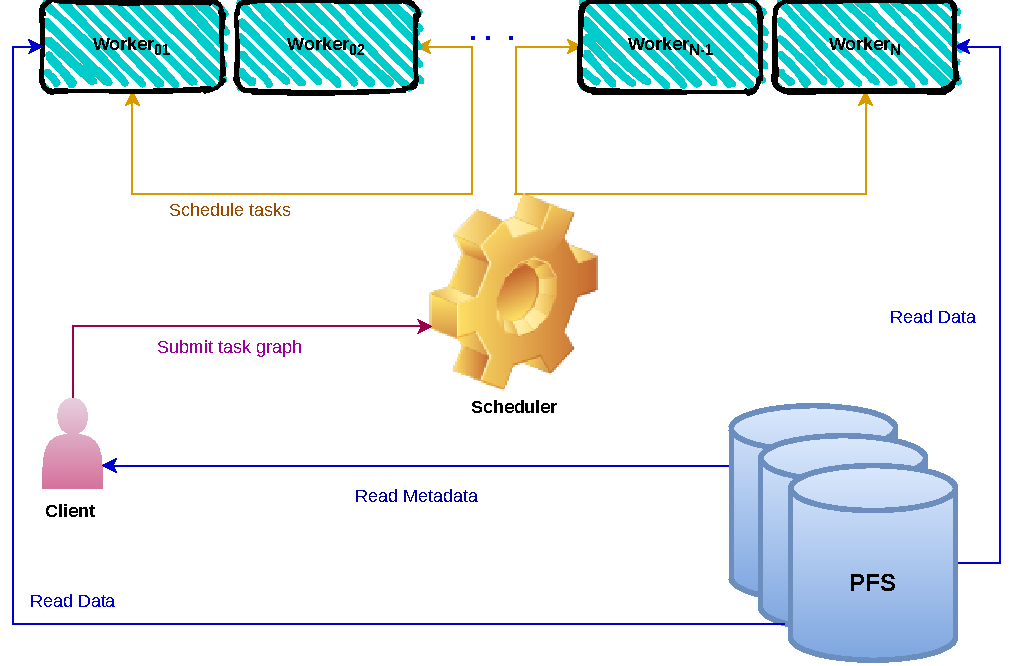
\includegraphics[scale=0.6]{figures/DaskArchiecture.pdf}
\caption{\dask distributed architecture in a typical post hoc context, one client and $N$ workers connected to the scheduler. 1) The client reads small metadata regarding the needed files from the PFS, 2) creates the \dask data structure and submits a task graph, 3) the workers execute the tasks, 4) some of them read data blocks in parallel from the PFS}
\label{figdaskarchi}
\end{figure}

\subsubsection{\dask Collections and Futures}
\amal{examples :)}
Among other advantages, \dask supports parallel versions of familiar libraries such as \texttt{Numpy} and \texttt{Pandas}, respectively, \texttt{dask.array} and \texttt{dask.dataframe}, with almost similar APIs. 
Thus, they become usable in larger-than-memory problems. In this work, we have been particularly interested in \textit{dask.array}. 

A \textit{dask.array}\cite{rocklin_dask_2015} is a larger-than-memory numpy-like array, it is constructed by smaller blocks of \texttt{numpy} arrays called chunks. Operation in a \textit{dask.array} generate automatically a corresponding task graph, thus called a high-level collection. 

The user can use the \textit{delayed} API to customize and create his own task graph, it may be advantageous when the user has particular processing which is not covered by the high-level collections. 
Moreover, \dask implements a \texttt{future} API, which is immediate rather than lazy.



\subsubsection{Tasks in \dask Distributed}
A task is a central concept in \dask and all task-based frameworks; it is the smallest piece of work that can be submitted to the scheduler and run by a worker. 

In this part, we will detail this concept in \dask, starting with task graph creation, the task state transition, and finally the task scheduling. We will define and discuss the \textit{pure data tasks} and how they were used in our work.



\paragraph{Task Graph}\label{sec:taskgraph}

Every script submitted to \dask scheduler is translated first to a task graph, specifically a directed acyclic graph of tasks with data dependencies. The graph is represented as a dictionary, where the keys are any hashable value that is not a task, and the values are computations. 

A task is a tuple that has a callable as a first element, followed by a list of arguments, and an argument may be any valid computation. A computation may be a key present in the graph, a value such as an integer, a task, or a list of computations. For instance \texttt{('function1', arg1, arg2, arg3)} is a task that applies \texttt{'function1'} to \texttt{(arg1, arg2, arg3)} where the arguments are valid computations such as: \texttt{{arg1: 1, arg2: ('function2', arg4), arg3: [('function3', arg5, 0.2), 5]}}.

The task \texttt{('function1', arg1, arg2, arg3)} is equivalent to run \texttt{function1(arg1, arg2, arg3)}, by moving the opening parenthesis one term to the left, the execution of \texttt{function1} is delayed. This representation allows \dask to store this computation as data that can be analyzed by the scheduler later rather than cause immediate execution.   

\paragraph{Task journey}

Task graph creation is not the only step that is done before getting to the scheduler.
Either the graph is constructed using high-level APIs or \texttt{Delayed} it goes through the following steps:
\begin{itemize}
    \item graph creation: as already presented in~\ref{sec:taskgraph}, the graph is encoded using a python dictionary, and it may include millions of entries. This step is done on the client side, 
    \item graph optimization: \dask tries to optimize the graph and eliminate unnecessary work. This may take some time if the graph is large,
    \item graph serialization: the graph needs to be sent from the client to the scheduler and then to the workers, so it must be converted into bytes before sending it. This is done in the serialization step. 
    \item graph communication: once the graph is serialized on the client side, it is sent to the scheduler.
\end{itemize}
These steps are done after calling the \texttt{compute/persist} and may take some time if the graph is very large. 
Now that the task graph is on the scheduler side, it populates its internal data structures to be able to analyze and schedule the tasks efficiently in the workers.

\paragraph{Task states}
In the \dask scheduler, a task can be in one of these 6 states: \texttt{"released", "waiting", "no-worker", "processing", "erred", "memory"}. It can move from one to another following stimulus coming either from a client or a worker. Figure~\ref{figdasktaskstate} shows the different states and transitions in \dask. 

\begin{figure}[tb]\centering
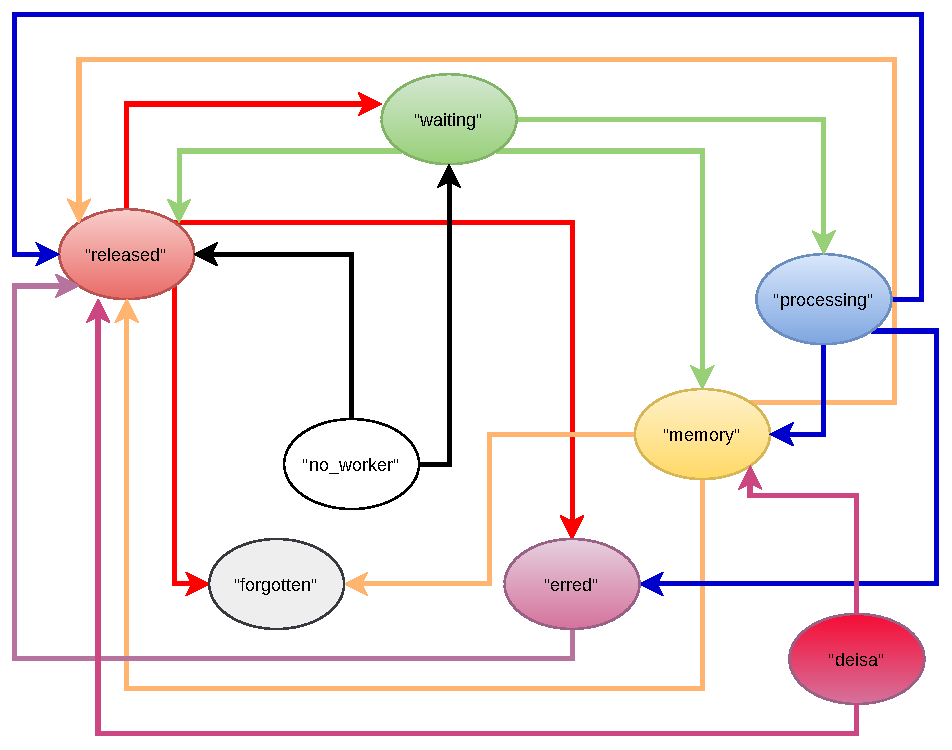
\includegraphics[scale=0.8]{figures/TaskStatesSheduler.pdf}
\caption{\dask task states and transitions \amal{it has been changed since then, \dask documentation and the code, but I still have the old version of \dask :p}}
\label{figdasktaskstate}
\end{figure}

When a task is created, it is in the state \texttt{"released"} which means that is known to the scheduler but not actively computing or in memory. It can pass to the \texttt{"waiting"} state that indicates that this task is waiting for dependencies to arrive in memory. It may also pass to the \texttt{"erred"} state if a depending task erred and to the \texttt{"forgotten"} state if it is not anymore needed by an alive client or dependent task. The \texttt{"no\_worker"} state means that the task is ready to be executed, but there is no worker connected, or no appropriate worker is available. 
A task in the \texttt{"waiting"} state passes the \texttt{"processing"} state when all its dependencies are in memory, and it is assigned to a worker to be computed. If it has been completed correctly, then it passes to the \texttt{"memory"} state. 

The \texttt{"deisa"} has been added in the frame of this work, and it represents external pure data tasks that are arrays of data generated by a running program, more details about this state will be found in the next sections. 

\subsubsection{Pure Data Tasks}\label{sec:puredata}
As already mentioned, usually, the source of the data in \dask is a storage system. However, it is possible for a client to send data to connected workers, either by passing by the scheduler or not. This can be done using the existing method in the client API \texttt{scatter}. The \texttt{scatter} function takes as a mandatory parameter: the data that needs to be sent, and other optional parameters such as a boolean that expresses whether or not to pass by the scheduler and a list of workers to whom the data will be sent. 
\texttt{scatter} returns a \texttt{future} to that data. The key of this \texttt{future} is the key of the equivalent pure data task in the \dask scheduler. That is, the data which is sent via a \texttt{scatter} is also a task.


\subsubsection{Scheduler Internal State}\label{sec:scheduler}

The scheduler keeps track of the tasks, alive clients and connected workers in its internal data structures that consist of four main objects: the \texttt{SchedulerState}, \texttt{TaskState}, \texttt{ClientState} and \texttt{WorkerState}
The \texttt{SchedulerState} object contains a global view of the internal state and uses the different classes. The \texttt{TaskState} keeps the state of each task (key, state, dependencies, dependents, ...), \texttt{ClientState} and \texttt{WorkerState} keep the state of a client and a worker, respectively.
Figure~\ref{figdaskinternal} shows the four main classes in the \dask scheduler internal state. 

\begin{figure}[tb]\centering
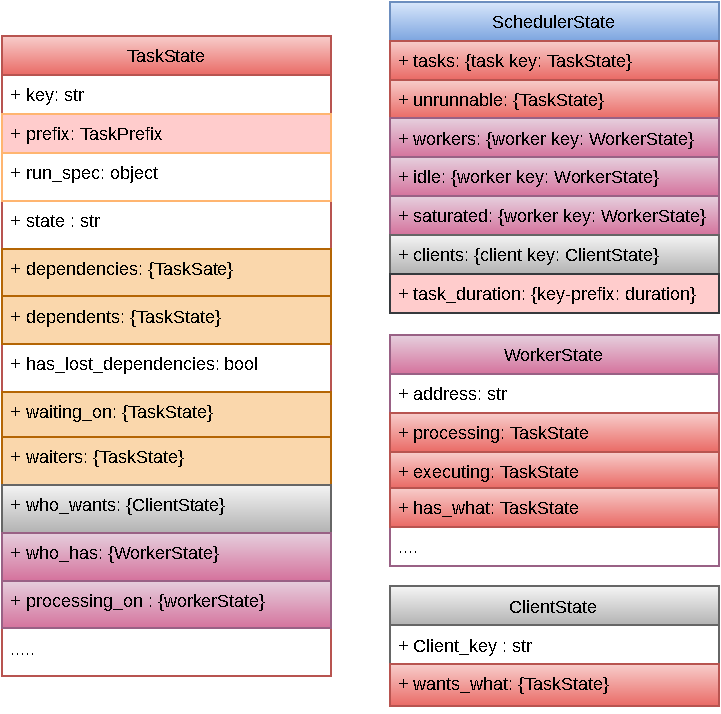
\includegraphics{figures/DaskScheduler.pdf}
\caption{\dask internal classes \amal{move to the implementation section maybe}}
\label{figdaskinternal}
\end{figure}

\subsubsection{Scheduling in \dask Distributed}\label{sec:scheduling}
In this section, we will not discuss the scheduling policies in \dask as it is not in the frame of this work. We will devote it to the \texttt{transition} algorithm, which performs state transition.
A task state transition occurs from stimuli, which are state-changing messages from workers and clients to the scheduler. 
The schedule handles those messages by triggering a \texttt{transition} function. Every state transition is implemented as a separate method in the scheduler, for instance, \texttt{transition\_processing\_memory} is the name of the function that performs the transition from the \textit{"processing"} to the \texttt{"memory"} state.

When a transition function is called, it mainly changes the state of the given task and constructs a dictionary of recommendations for the state transitions of other tasks. In addition to the specific transition functions, there is the \texttt{transitions} that is called, as its name indicates, it triggers several transitions by iterating over the recommendations. 

For example, when the scheduler receives the \texttt{"task-finished"} stimuli. The \texttt{transition\_processing\_memory} is called, it switches the task state from \texttt{"processing"} to \texttt{"memory"} and recommends all dependent tasks to switch to the \texttt{"processing"} state. These recommendations are passed then to the \texttt{transitions} function that iterates over until no more recommendation is added.

A set of messages to the clients and the workers is also constructed and sent. For instance, those may contain results needed by a client or a task to be run by a worker.

\amal{pseudo algo?}

\subsection{\pdi}\label{sec:pdi}
\subsubsection{Overview}\label{sec:pdioverview}

\pdi\cite{roussel:hal-01587075} data interface is a lightweight library for data handling. It separates simulation core concerns from cross-cutting concerns. It proposes a declarative way to call external libraries from a configuration file rather than inline the calls in the simulation codes. 
PDI is built around three core concepts: 
\begin{itemize}
    \item data store: when data is shared from the simulation, it is made available to \pdi through the data store,
    \item event subsystem: once the data is available in the data store, the event system notifies the data handler plugin,
    \item plugins: they access the data available in the store and process it.   
\end{itemize}
The data layout, the orchestration of the exchanges, and the configuration of the different plugins are described in the specification tree; figure~\ref {figpdiarchi} shows a structure scheme of \pdi\cite{noauthor_pdi_nodate}.  


\begin{figure}[tb]\centering
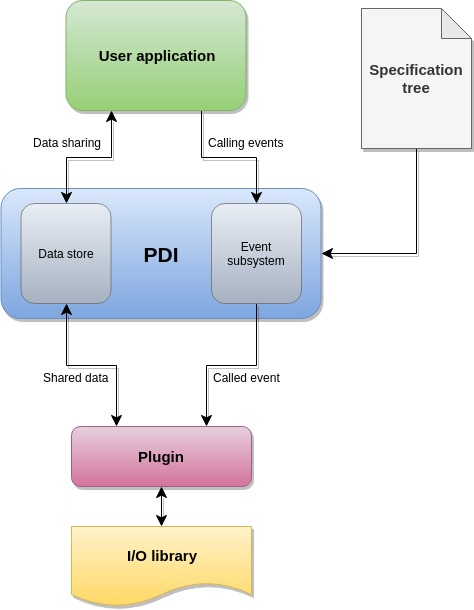
\includegraphics[scale=0.5]{figures/PDI_schema.jpg}
\caption{\pdi architecture\cite{PDI}}
\label{figpdiarchi}
\end{figure}

\subsubsection{\pdi API and Simulation Instrumentation}
\pdi offers a very simple API; its functions can be grouped into three categories. The initialization and finalization functions respectively \texttt{PDI\_init} and \texttt{PDI\_finalize} are used to setup and finalize PDI by releasing its resources. 
The second category consists of a set of functions used to annotate the code. \texttt{PDI\_share}, \texttt{PDI\_reclaim} are use to respectively share data with \pdi and reclaim it. \texttt{PDI\_expose} does both sharing and reclaiming the data from the data store. \textit{PDI\_event} triggers a PDI event and finally, \texttt{PDI\_multi\_expose} exposes several variables and triggers an event. Listing~\ref{ccode} shows an example of a c code instrumentation with \pdi, \pdi API calls are highlighted.

\begin{lstlisting}[float, label=ccode, language=c, caption=\pdi instrumentation of the C simulation code]
int main( int argc, char* argv[] ) {
  MPI_Init(&argc, &argv);
  |\hlline|PDI_init(PC_parse_path("pdi_spec.yml")); |\label{ccode:PDI_init}|
  int rank; PDI_Comm_rank(MPI_COMM_WORLD, &rank);
  config_t cfg = read_config("simulation.yml");
  // share one-off configuration
  |\hlline|PDI_multi_expose("init", |\label{ccode:expose1}|
  |\hlline|    "cfg",  &cfg,  PDI_OUT, |\label{ccode:cfg}|
  |\hlline|    "rank", &rank, PDI_OUT,
  |\hlline|    NULL); |\label{ccode:expose1-end}|
  // our temperature field
  double* temp = malloc(sizeof(double) * cfg.loc[0] * cfg.loc[1]);
  initialize(temp);
  // main loop
  for (int step=0; ii<nb_steps; ++step) {
    do_compute(temp, MPI_COMM_WORLD);|\label{ccode:compute}|
    // share data at every iteration
    |\hlline|PDI_multi_expose("iter",  |\label{ccode:expose2}|
    |\hlline|    "step", &step, PDI_OUT,
    |\hlline|    "temp", temp,  PDI_OUT,
    |\hlline|    NULL); |\label{ccode:expose2-end}|
    MPI_Barrier(MPI_COMM_WORLD);|\label{ccode:barrier}|
  }
  free(temp);
  |\hlline|PDI_finalize();
  MPI_Finalize();
}
\end{lstlisting}

\subsubsection{\pdi Specification Tree}
As already mentioned in the \ref{sec:pdioverview}, the specification tree describes the data layout, orchestrates the interactions between the code and \pdi, and contains the plugin's configurations. It is specified in a \texttt{yaml} file and is provided to \pdi at the initialization, for instance, in listing~\ref{ccode} line\ref{ccode:PDI_init} the configuration file name is \texttt{"pdi\_spec.yml"}. 

The specification tree contains three mains sections: the \texttt{metadata}, the \texttt{data} and the \texttt{plugins} section. The \texttt{metadata} section contains small variables whose \pdi keeps a copy of, and it may contain, for example, the sizes of a given array. The \texttt{data} section contains the data layout description. It defines the types of data expected in the store. Those data are not copied by \pdi; only pointers to the data are shared. Finally, the \texttt{plugins} section lists the plugins that will be loaded and their configurations. 

Listing~\ref{pdiymldata} shows an example of a \pdi \texttt{yaml} configuration file where a \texttt{types} section is added, where we can define new types such as \texttt{structures}. In this example we find also the \texttt{metadata} section in line~\ref{pdiymldata:metadata}. The \texttt{data} section starts in line~\ref{pdiymldata:data}, it provides a description of the \texttt{temp} field, (line~\ref{pdiymldata:temp}) including its type, subtype and size (respectively in lines~\ref{pdiymldata:temp.type},~\ref{pdiymldata:temp.subsize},~\ref{pdiymldata:temp.size}). 
Finally, the \texttt{plugin} section starts in line~\ref{pdiymldata:plugin}, it loads one plugin: the \texttt{decl\_hdf5} plugin in line~\ref{pdiymldata:declhdf5}. We will detail the \pdi plugin system in section~\ref{plugins}.

\begin{lstlisting}[float, label=pdiymldata, language=yaml, caption=Data description in \pdi YAML file]
types: #[...] including config_t description
metadata: {step: int, cfg: config_t, rank: int} |\label{pdiymldata:metadata}|
data: |\label{pdiymldata:data}|
  temp: # the main temperature field |\label{pdiymldata:temp}|
    type: array |\label{pdiymldata:temp.type}|
    subtype: double |\label{pdiymldata:temp.subsize}|
    size: [ '$cfg.loc[0]', '$cfg.loc[1]' ]  |\label{pdiymldata:temp.size}|
plugins: |\label{pdiymldata:plugin}|
  decl_hdf5: |\label{pdiymldata:declhdf5}|
  - file: data-$step-$rank.h5 
    write:
      temp:
        when: '$step>0' |\label{pdiymldata:when}|
\end{lstlisting}

\subsubsection{\pdi Plugins}\label{plugins}
\pdi supports loose coupling of simulation codes with libraries. Those libraries are supported in \pdi as plugins and are configured through the specification tree. \pdi offers a list of built-in plugins ranging from IO-specific ones to more generic data handling tools. It also allows the creation of user-specific plugins if the built-in ones are not enough.     

\paragraph{Built-in Plugins}
The built-in plugins \pdi provides can be grouped into four categories: 
\begin{itemize}
    \item general purpose: include \texttt{mpi}, \texttt{trace}, \texttt{set\_value}.  
    \item trace and debugging: include \texttt{trace} plugin,
    \item IO: include \texttt{decl’hdf5}, \texttt{decl’NetCDF}, \texttt{SIONlib} plugins
    \item fault tolerance: \texttt{FTI}plugin.
\end{itemize}

In listing~\ref{pdiymldata}, one plugin have been used the \texttt{decl\_hdf5} plugin in line~\ref{pdiymldata:declhdf5}. In this example, a file named \textit{data-step-rank.h5} is written by each process in every step greater than 0. The \texttt{\$-expression} gets the actual value of \texttt{rank} and \texttt{step}.    

\paragraph{User-defined Plugins}
\pdi is extensible, and the user can add his own plugins. For instance, a \texttt{FlowVR} and a \texttt{Melissa} plugin have been added. \texttt{FlowVR}\cite{} is a middleware based on dataflow paradigm for in situ processing and \texttt{Melissa}\cite{} is an in situ framework for sensibility analysis. In the same context of in situ analytics, a plugin for \texttt{sensei} has been developed, and in this work, we have implemented a new plugin to interface with \dask called \deisa plugin.  




